% OUTPUT MODALITIES
% using the tablet PC's display
% using a powerwall
% using HMDs

In order to obtain an immersive experience, there's a number of hardware
setups commonly available:

\begin{description}
	\item[Head-Mounted Display (HMD)] --
	  Head-mounting displays are glass-shaped devices, projecting a pair of stereo
	  transformed images to the user's retinas.
	  They normally feature a gyroscope or similar apparatus to measure head orientation and tilt.
	  There are two kinds of HMDs: in the former the images are projected in small opaque screens;
	  in the latter the projected surface is translucid, allowing blending of real and virtual worlds.
	  Translucid HMDs are best crafted for Augmented Reality (AR).
	  
		Using an HMD has the benefit of sticking to the user's head and detecting head orientation.
		On the other hand each HMD serves one single user and it has limited resolution.
		Additionally, most users report suffering from fatigue after long periods of
		usage \cite{VREDUC}.
		Opaque HMDs have the additional downside of users being unable to see the real world, 
		which can be confusing as noted by \cite{VANDERPOL}.
			
	\item[Cave Automatic Virtual Environment (CAVE)] --
	  A CAVE is an immersive virtual reality environment where projectors are directed to four,
	  five or all the six walls of a room-sized cube.
	  
		It shares the benefit of enclosing the user's viewing area with HMDs.
		Has a better resolution though.
		The downside is the small number of simultaneous users who can experience the CAVE at the same time.
	
	\item[Power Wall] --
	  A power wall is a large surface, usually planar, filled by an image.
	  The whole image projection is responsibility of a cluster of projectors set up in a wall.
	  Each projector renders part of the surface and the border between projections is ideally minimal.
	  Each projector is controlled by an independent computer.
	  
		Its size and resolution depend entirely on the setup, but normally a wall offers high resolution
		(depends on the number of projectors in the grid and each projector's resolution).
		Due to the large surface of the wall, several users may be served as once. Another benefit
		is users freedom of movement due to users not carrying wires \cite{INTTABLE}.
		The downside is users having to face the wall to experience the image entirely.
\end{description}

\begin{figure}[!ht]
	\centering
	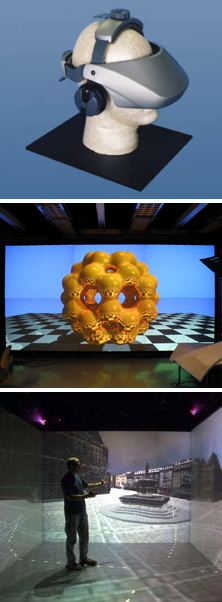
\includegraphics[width=12cm]{gfx/hmd-cluster-cave.png}
	\caption{HMD, Wall, CAVE}
	\label{FIG-HMD-CLUSTER-CAVE}
\end{figure}

Any of these setups is suitable for single user interaction.
In case of a reviewing session, in which at least two participants are required,
CAVE or Wall are better suited, since they alone offer a solution for a small group.

Using a Wall or CAVE presents other challenges: the computers responsible for
generating each projectors' images must be synchronized, its color parameters calibrated
and the viewport must be well cropped.
Several systems exist capable of delivering high performance 3D graphics and
offering the features mentioned above.
Based on scene graphs there are two well established solutions:
OpenSceneGraph\cite{SITE-OSG} and OpenSG\cite{SITE-OPENSG}.
